\chapter{Statistical Testing}\label{chap:stat_testing}
Inspired by \cite{hexeberg}, the performance of the proposed models will be compared on straight-line and curved trajectories independently.

\section{Method}
\subsection{Trajectory Error}
The trajectory error is found by comparing the predicted position with the ground truth. As the predicted trajectory is simulated in discrete time, the points with the closest timestamps are used for comparison. With $\Delta T = 10\text{ seconds}$, the maximum error in time is $\frac{\Delta T}{2} = 5 \text{ seconds}$, which is considered to be acceptable considering the time-horizon of between $15$ and $30$ minutes.
\subsection{Path Error}
The path error is defined as the closest point in the predicted trajectory to each point in the ground truth, under the constraint that the corresponding predicted timestamps must be monotonically increasing. In other words, the path cannot move backward in time. Linear interpolation is used to get the path error at fixed timestamps to simplify the comparison.

\subsection{Normalized Estimation Error Squared}
For the uncertainty estimates to provide any value, the predictions must be consistent. In this context, the term consistency is borrowed from the term \textit{filter consistency} used when tuning Kalman filters \cite{sensorfusjon}. The idea is that prediction errors, on average, should scale with the state covariance. In other words, the model should not place a lot of confidence in a prediction that is wrong while being highly confident when a prediction is correct. Consistency can also be interpreted using a frequentistic interpretation of probability, where after many predictions, the state uncertainty should reflect the actual error rate.

The \textit{\acrfull{nees}} is a metric that can be used to quantify consistency and is given by
\begin{equation}
    \text{NEES} = (\boldsymbol{x} - \hat{\boldsymbol{x}})^\intercal \boldsymbol{P}^{-1} (\boldsymbol{x} - \hat{\boldsymbol{x}})
\end{equation}

Assuming the prediction error follows a Gaussian distribution, the \acrshort{nees} follows a Chi-Squared distribution which can be used to form a confidence interval. Comparing the prediction errors with this confidence interval can then be used to get a sense of whether the estimated state uncertainty is consistent with the actual error rate.

\subsection{Interpolation}
Linear interpolation is used to compare the metrics at fixed timestamps between samples. The error for short trajectories is not extrapolated.

\subsection{Baseline - Constant Velocity Model}
As a basis of comparison, the \textit{\acrfull{cvm}} method is used as a baseline. The model uses the initial \acrshort{cog} and \acrshort{sog} to predict a straight line, where the vessel is assumed to keep a constant velocity and heading.

\subsection{Sanitizing the dataset for a given test trajectory}
Due to the way trajectories are generated from the \acrshort{ais} dataset, there will be large overlaps between trajectories. Dividing the trajectories into a train and test is insufficient, as parts of a test trajectory might also exist in the training set. Instead, the full dataset is available for training, but all trajectories with identical MMSI and date as the test trajectory are removed. The date requirement ensures that trajectories for the same vessel can be used for training on any other day.

\subsection{Straigth-line trajectories}
The GP-EKF is first compared to the \acrshort{cvm} on simple straight-line trajectories. The GP-EKF should ideally perform identically or better than the \acrshort{cvm}.
The statistics are based on $350$ randomly sampled trajectories without replacement that satisfy the following requirements:
\begin{enumerate}
    \item The sum of subsequent changes in \acrshort{cog} must be less than $30$ degrees, i.e. $\sum_i |(\mathcal{X}_{t+1} - \mathcal{X}_t)| \leq 30^\circ$. This requirement ensures a straight-line trajectory.
    \item There must be sufficient data available for training in the neighborhood around the initial starting point, with similar initial heading and speed. After sanitizing the dataset and removing irrelevant trajectories, at least $3$ trajectories need to be available for training.
    \item The overall duration of the trajectories must be between $15$ and $30$ minutes.
\end{enumerate}




\subsection{Curved Trajectories}
The GP-EKF is then compared to the \acrshort{cvm} on curved trajectories. The GP-EKF should ideally perform drastically better than the \acrshort{cvm}.
The statistics are based on $350$ randomly sampled trajectories that satisfy the following requirements:
\begin{enumerate}
    \item The sum of subsequent changes in \acrshort{cog} must be greater than $40$ degrees, i.e. $\sum_i |(\mathcal{X}_{t+1} - \mathcal{X}_t)| \geq 40^\circ$. This requirement ensures a straight-line trajectory.
    \item There must be sufficient data available for training in the neighborhood around the initial starting point, with similar initial heading and speed. After sanitizing the dataset and removing irrelevant trajectories, at least $3$ trajectories need to be available for training.
    \item The overall duration of the trajectories must be between $15$ and $30$ minutes.
\end{enumerate}


\section{The Methods}
Both the direct \acrshort{gp} and the GP-EKF are used for testing.

\subsection{GP-EKF}
The GP-EKF is tested with and without the \acrshort{pdaf} update step to test whether there is any benefit of using the update step. The model is tested using both finite difference and the \acrshort{cog}/\acrshort{sog} from the \acrshort{ais} dataset. $4$ different GP-EKF instants are therefore included in this test.

\subsection{Direct GP}
Only the representable subset approach of the direct \acrshort{gp} approach is included in this testing for two reasons:
\begin{enumerate}
    \item All methods can use the same representative trajectories for training. As a result, it becomes easier to compare the different methods as the performance is not influenced by how the training data is selected.
    \item The \acrshort{svgp} turned out to be very complicated to make work. Even after several hours of training, the model performed rather poorly, with unrealistic trajectory estimates. It was therefore decided that it was not worth the additional effort.
\end{enumerate}

\section{Results}
The results for straight-line and curved trajectories are available in \cref{table:stats_straight_line_error} and \cref{table:stats_curved_error} respectively. \todo[]{add examples in appendix?}. As expected, the \acrshort{cvm} method performs well on the straight-line trajectories, while struggles on the curved trajectories.
\begin{table}
    \begin{subtable}{\textwidth}
        \makebox[\textwidth][c]{
            \begin{tabular}{lllrrrrr}
                \toprule
                        &                & Time [Minutes]    & 5   & 10   & 15   & 20   & 25   \\
                Summary & Method         & Training Source   &     &      &      &      &      \\
                \midrule
                Mean    & CVM            & COG/SOG from AIS  & 674 & 1347 & 2024 & 2332 & 2272 \\
                        & Direct GP      & Position          & 969 & 1319 & 1838 & 2557 & 2845 \\
                        & GP-EKF         & COG/SOG from AIS  & 590 & 1169 & 1678 & 1883 & 2318 \\
                        &                & Finite Difference & 562 & 1078 & 1645 & 2400 & 2560 \\
                        & GP-EKF w/ PDAF & COG/SOG from AIS  & 596 & 1149 & 1618 & 1848 & 2207 \\
                        &                & Finite Difference & 568 & 1059 & 1603 & 2323 & 2448 \\
                \midrule
                Median  & CVM            & COG/SOG from AIS  & 481 & 968  & 1538 & 1863 & 2073 \\
                        & Direct GP      & Position          & 549 & 892  & 1295 & 1896 & 2529 \\
                        & GP-EKF         & COG/SOG from AIS  & 445 & 888  & 1258 & 1373 & 2402 \\
                        &                & Finite Difference & 418 & 682  & 1140 & 1591 & 1841 \\
                        & GP-EKF w/ PDAF & COG/SOG from AIS  & 443 & 866  & 1203 & 1353 & 2367 \\
                        &                & Finite Difference & 427 & 683  & 1108 & 1503 & 1736 \\
                \bottomrule
            \end{tabular}
        }
        \caption{Trajectory errors in meters}
        \label{table:stats_straight_traj_err}
        \vspace*{0.5cm}
    \end{subtable}
    \begin{subtable}{\textwidth}
        \makebox[\textwidth][c]{
            \begin{tabular}{lllrrrrr}
                \toprule
                        &                & Time [Minutes]    & 5   & 10  & 15   & 20   & 25   \\
                Summary & Method         & Training Source   &     &     &      &      &      \\
                \midrule
                Mean    & CVM            & COG/SOG from AIS  & 142 & 497 & 1144 & 1550 & 2033 \\
                        & Direct GP      & Position          & 487 & 534 & 806  & 1412 & 2195 \\
                        & GP-EKF         & COG/SOG from AIS  & 218 & 483 & 949  & 1183 & 1408 \\
                        &                & Finite Difference & 229 & 460 & 745  & 1249 & 1042 \\
                        & GP-EKF w/ PDAF & COG/SOG from AIS  & 209 & 442 & 867  & 1118 & 1298 \\
                        &                & Finite Difference & 222 & 428 & 692  & 1173 & 957  \\
                \midrule
                Median  & CVM            & COG/SOG from AIS  & 70  & 262 & 703  & 1206 & 1971 \\
                        & Direct GP      & Position          & 181 & 310 & 429  & 782  & 2186 \\
                        & GP-EKF         & COG/SOG from AIS  & 142 & 310 & 602  & 785  & 959  \\
                        &                & Finite Difference & 143 & 277 & 375  & 700  & 743  \\
                        & GP-EKF w/ PDAF & COG/SOG from AIS  & 145 & 284 & 515  & 742  & 841  \\
                        &                & Finite Difference & 146 & 250 & 357  & 646  & 761  \\
                \bottomrule
            \end{tabular}
        }
        \caption{Path error in meters}
        \label{table:stats_straight_path_err}
    \end{subtable}
    \caption{Error summary for $350$ straight-line trajectories. Mean and median summary statistics are calculated for the trajectory and path error at fixed timestamps. Linear interpolation is used between samples. Errors for short trajectories are not extrapolated, and therefore not included in the $20$ and $25$ minute bins.}
    \label{table:stats_straight_line_error}
\end{table}

\begin{table}
    \begin{subtable}{\textwidth}
        \makebox[\textwidth][c]{
            \begin{tabular}{lllrrrrr}
                \toprule
                        &                & Time [Minutes]    & 5    & 10   & 15   & 20    & 25    \\
                Summary & Method         & Training Source   &      &      &      &       &       \\
                \midrule
                Mean    & CVM            & COG/SOG from AIS  & 1282 & 3238 & 6127 & 10066 & 14604 \\
                        & Direct GP      & Position          & 490  & 736  & 889  & 893   & 979   \\
                        & GP-EKF         & COG/SOG from AIS  & 787  & 1614 & 2331 & 2909  & 3520  \\
                        &                & Finite Difference & 709  & 1392 & 1835 & 2242  & 2380  \\
                        & GP-EKF w/ PDAF & COG/SOG from AIS  & 722  & 1449 & 1986 & 2290  & 2310  \\
                        &                & Finite Difference & 724  & 1355 & 1752 & 2098  & 2233  \\
                \midrule
                Median  & CVM            & COG/SOG from AIS  & 875  & 2605 & 5419 & 10325 & 15008 \\
                        & Direct GP      & Position          & 233  & 381  & 479  & 531   & 644   \\
                        & GP-EKF         & COG/SOG from AIS  & 614  & 1258 & 1949 & 2521  & 3603  \\
                        &                & Finite Difference & 512  & 982  & 1582 & 2049  & 2162  \\
                        & GP-EKF w/ PDAF & COG/SOG from AIS  & 525  & 1101 & 1461 & 1457  & 1829  \\
                        &                & Finite Difference & 534  & 922  & 1527 & 1890  & 2168  \\
                \bottomrule
            \end{tabular}
        }
        \caption{Trajectory Error in meters}
        \label{table:stats_curved_traj_err}
        \vspace*{0.5cm}
    \end{subtable}
    \begin{subtable}{\textwidth}
        \makebox[\textwidth][c]{
            \begin{tabular}{lllrrrrr}
                \toprule
                        &                & Time [Minutes]    & 5   & 10   & 15   & 20   & 25   \\
                Summary & Method         & Training Source   &     &      &      &      &      \\
                \midrule
                Mean    & CVM            & COG/SOG from AIS  & 484 & 1383 & 2793 & 4494 & 6105 \\
                        & Direct GP      & Position          & 323 & 409  & 456  & 514  & 662  \\
                        & GP-EKF         & COG/SOG from AIS  & 267 & 671  & 1383 & 2046 & 2870 \\
                        &                & Finite Difference & 400 & 615  & 742  & 723  & 565  \\
                        & GP-EKF w/ PDAF & COG/SOG from AIS  & 259 & 565  & 1054 & 1466 & 1678 \\
                        &                & Finite Difference & 412 & 594  & 704  & 682  & 538  \\
                \midrule
                Median  & CVM            & COG/SOG from AIS  & 188 & 776  & 1867 & 3671 & 6797 \\
                        & Direct GP      & Position          & 92  & 161  & 180  & 192  & 276  \\
                        & GP-EKF         & COG/SOG from AIS  & 114 & 323  & 863  & 1340 & 2555 \\
                        &                & Finite Difference & 227 & 398  & 481  & 437  & 344  \\
                        & GP-EKF w/ PDAF & COG/SOG from AIS  & 130 & 264  & 512  & 789  & 916  \\
                        &                & Finite Difference & 274 & 389  & 458  & 403  & 363  \\
                \bottomrule
            \end{tabular}
        }
        \caption{Path error in meters}
        \label{table:stats_curved_path_err}
    \end{subtable}
    \caption{Error summary for $350$ curved trajectories. Mean and median summary statistics are calculated for the trajectory and path error at fixed timestamps. Linear interpolation is used between samples. Errors for short trajectories are not extrapolated, and therefore not included in the $20$ and $25$ minute bins.}
    \label{table:stats_curved_error}
\end{table}


\subsection{Comparing Direct GP to CVM}
\begin{figure}[h]
    \centering
    \makebox[\textwidth][c]{
        \begin{subfigure}{0.65\textwidth}
            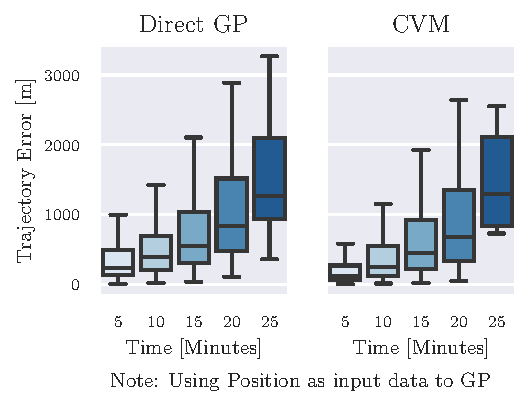
\includegraphics[width=\textwidth]{figures/straight_line_stats/gp_vs_cvm_1.pdf}
            \caption{Straight-Line Trajectories}
        \end{subfigure}
        \begin{subfigure}{0.65\textwidth}
            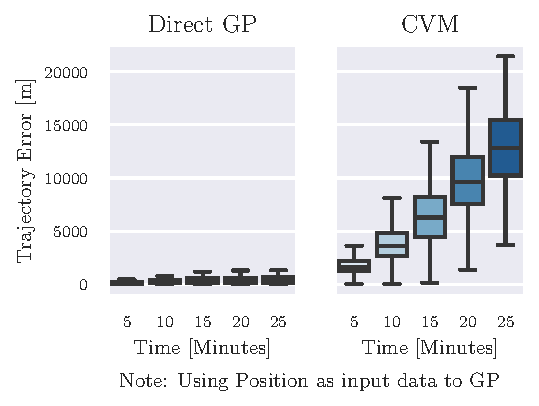
\includegraphics[width=\textwidth]{figures/curved_line_stats/gp_vs_cvm_1.pdf}
            \caption{Curved Trajectories}
        \end{subfigure}
    }
    \caption{GP-EKF compared to the CVM method on $350$ random trajectories. As expected, the \acrshort{cvm} yields large trajectory errors on curved trajectories. The GP-EKF performs consistently better, with lower median error as well as lower spread. However, on straight-line trajectories, the methods behave comparably.}
    \label{fig:stats_curved_posgp_cvm}
\end{figure}
The Direct GP approach performs slightly worse than the \acrshort{cvm} on straight-line trajectories, while it performs significantly better on curved trajectories, with overall lower spread and median trajectory error as depicted in \cref{fig:stats_curved_gp_ekf_cvm}.

\subsection{Comparing GP-EKF to CVM}
\begin{figure}[h]
    \centering
    \makebox[\textwidth][c]{
        \begin{subfigure}{0.65\textwidth}
            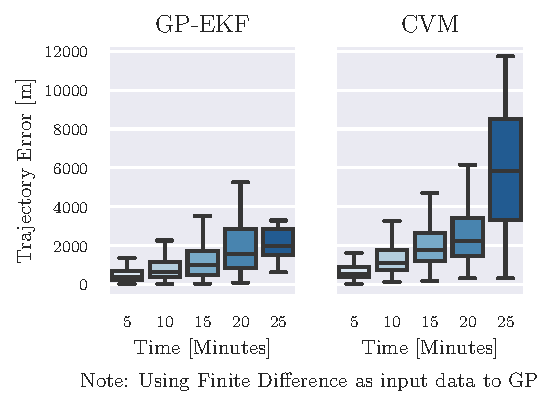
\includegraphics[width=\textwidth]{figures/straight_line_stats/gp_vs_cvm_3.pdf}
            \caption{Straight-Line Trajectories}
        \end{subfigure}
        \begin{subfigure}{0.65\textwidth}
            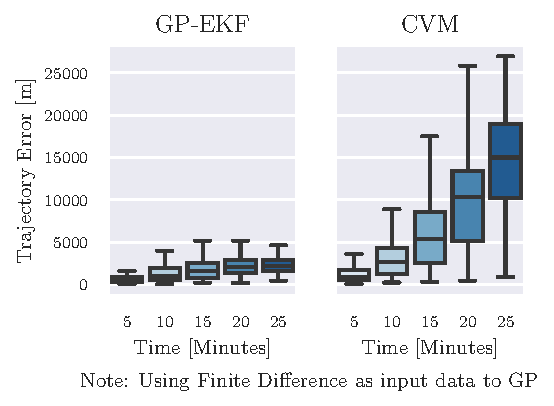
\includegraphics[width=\textwidth]{figures/curved_line_stats/gp_vs_cvm_3.pdf}
            \caption{Curved Trajectories}
        \end{subfigure}
    }
    \caption{GP-EKF compared to the CVM method on $350$ random trajectories. As expected, the \acrshort{cvm} yields large trajectory errors on curved trajectories. The GP-EKF performs consistently better, with lower median error as well as lower spread. However, on straight-line trajectories, the methods behave comparably.}
    \label{fig:stats_curved_gp_ekf_cvm}
\end{figure}
The GP-EKF approach performs significantly better than the \acrshort{cvm} on curved trajectories, with overall lower spread and median trajectory error as depicted in \cref{fig:stats_curved_gp_ekf_cvm}.

\subsection{Effect of the PDAF update}
\begin{figure}
    \centering
    \makebox[\textwidth][c]{
        \begin{subfigure}{0.65\textwidth}
            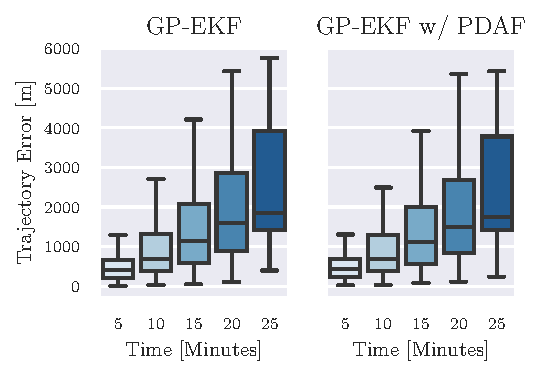
\includegraphics[width=\textwidth]{figures/straight_line_stats/gp_vs_pdaf.pdf}
            \caption{Straight-Line Trajectories}
        \end{subfigure}
        \begin{subfigure}{0.65\textwidth}
            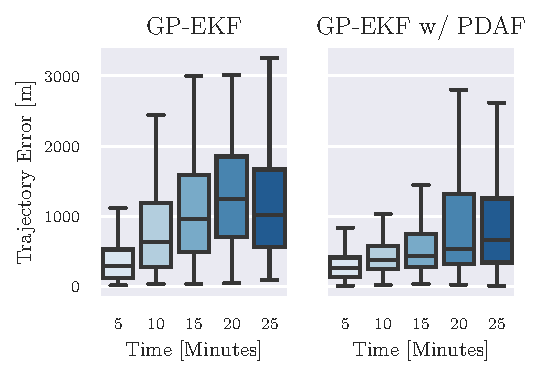
\includegraphics[width=\textwidth]{figures/curved_line_stats/gp_vs_pdaf.pdf}
            \caption{Curved Trajectories}
        \end{subfigure}
    }
    \caption{GP-EKF with and without PDAF on curved trajectories for $350$ trajectories. While there are some slight differences, the \acrshort{pdaf} does not appear to have any considerable effect on the trajectory errors.}
    \label{fig:stats_gp_ekf_with_or_without_pdaf}
\end{figure}

When comparing the performance of GP-EKF with and without the update step in \cref{fig:stats_gp_ekf_with_or_without_pdaf}, there seems to be little actual gain from the added complexity of \acrshort{pdaf}.


\subsection{Finite Difference vs. COG/SOG from AIS}
A key design choice for the GP-EKF is which data source to use for training. The model can either be trained using the \acrshort{cog} and \acrshort{sog} values contained in the \acrshort{ais} samples or by calculating numerical derivatives of the position through a finite-difference approach. Comparing trajectory error for both approaches on the same test set favors the finite-difference approach, as seen in \cref{fig:stats_curved_gp_ekf_fd_vs_cog}. The finite difference approach performs consistently better, with lower median error and less spread. However, by ignoring the time component, looking at the path errors in \cref{table:stats_curved_path_err} supports the opposite, where the path errors are lower for the \acrshort{cog}/\acrshort{sog} approach. This may indicate that the issue is due to imprecise velocity estimates from the \acrshort{sog} while using the course from the \acrshort{cog} works well.
\begin{figure}
    \centering
    \makebox[\textwidth][c]{
        \begin{subfigure}{0.65\textwidth}
            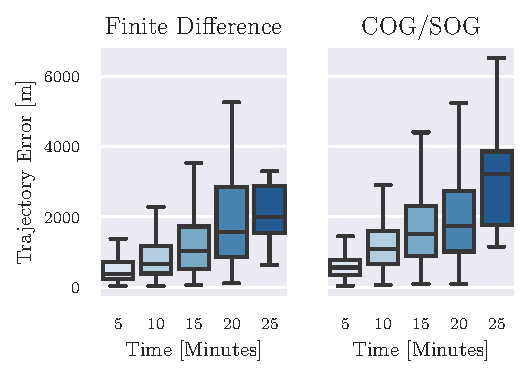
\includegraphics{figures/straight_line_stats/gp_cog_vs_fd.pdf}
            \caption{Straight-Line Trajectory}
        \end{subfigure}
        \begin{subfigure}{0.65\textwidth}
            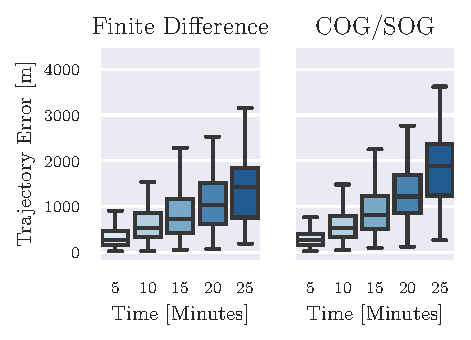
\includegraphics{figures/curved_line_stats/gp_cog_vs_fd.pdf}
            \caption{Curved Trajectory}
        \end{subfigure}
    }
    \caption{GP-EKF using finite differences and the \acrshort{cog} and \acrshort{sog} from the AIS dataset on $350$ trajectories. The finite differences approach performs consistently better, with lower median error and spread.}
    \label{fig:stats_curved_gp_ekf_fd_vs_cog}
\end{figure}


\section{Consistency}
\begin{figure}[h]
    \centering
    \makebox[\textwidth][c]{
        \begin{subfigure}{0.65\textwidth}
            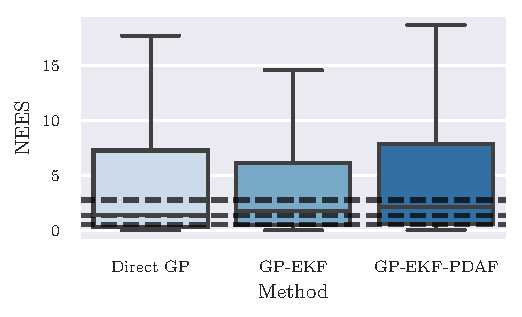
\includegraphics{figures/straight_line_stats/nees.pdf}
            \caption{Straight-Line Trajectory}
        \end{subfigure}
        \begin{subfigure}{0.65\textwidth}
            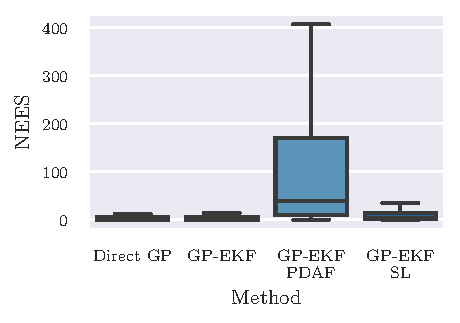
\includegraphics{figures/curved_line_stats/nees.pdf}
            \caption{Curved Trajectory}
        \end{subfigure}
    }
    \begin{subfigure}{0.65\textwidth}
        \centering
        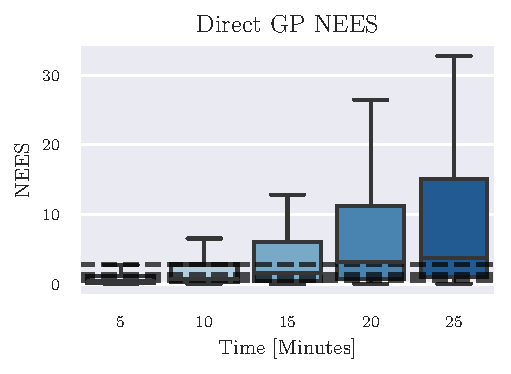
\includegraphics{figures/curved_line_stats/direct_gp_nees.pdf}
        \caption{Direct GP NEES for curved trajectories}
        \label{fig:stats_curved_nees_direct}
    \end{subfigure}
    \caption{Boxplot of the \acrshort{nees} on straight-line and curved trajectories for each method. The dotted lines shows the theoritical quartiles ($25\%$, $50\%$ and $75\%$) for the $\mathcal{X}^2$ distribution as a comparison.}.
    \label{fig:stats_curved_nees}
\end{figure}
The estimated quartiles \acrshort{nees} for straight-line and curved trajectories is displayed for each method in \cref{fig:stats_curved_nees}.

On straight-line trajectories, the $25\%$ and $50\%$ quartiles correspond well with the theoretical values for the $\mathcal{X}^2$ distribution for all methods. The \acrshort{pdaf} update step does, however, reduce the predicted uncertainty, leading to increased overconfidence. In addition, the estimated \acrshort{nees} distribution has a much fatter right-tail than the theoretical $\mathcal{X}^2$ distribution, leading to an estimated $75\%$ quartile far outside the theoretical values.

On curved trajectories, the GP-EKF with and without PDAF is consistently overconfident. The theoretical quartiles are not plotted due to the large y-axis. The direct \acrshort{gp} approach performs significantly better, which is why a separate plot in \cref{fig:stats_curved_nees_direct} is added to compare it to theoretical quartiles. 




